\subsection{Election November 5, 1996: *Clinton vs Dole}
\begin{frame}[t]{Election November 5, 1996: *Bill Clinton}
\small

\begin{columns}[T, onlytextwidth]
\column{0.48\textwidth}
\vspace{-1em}
{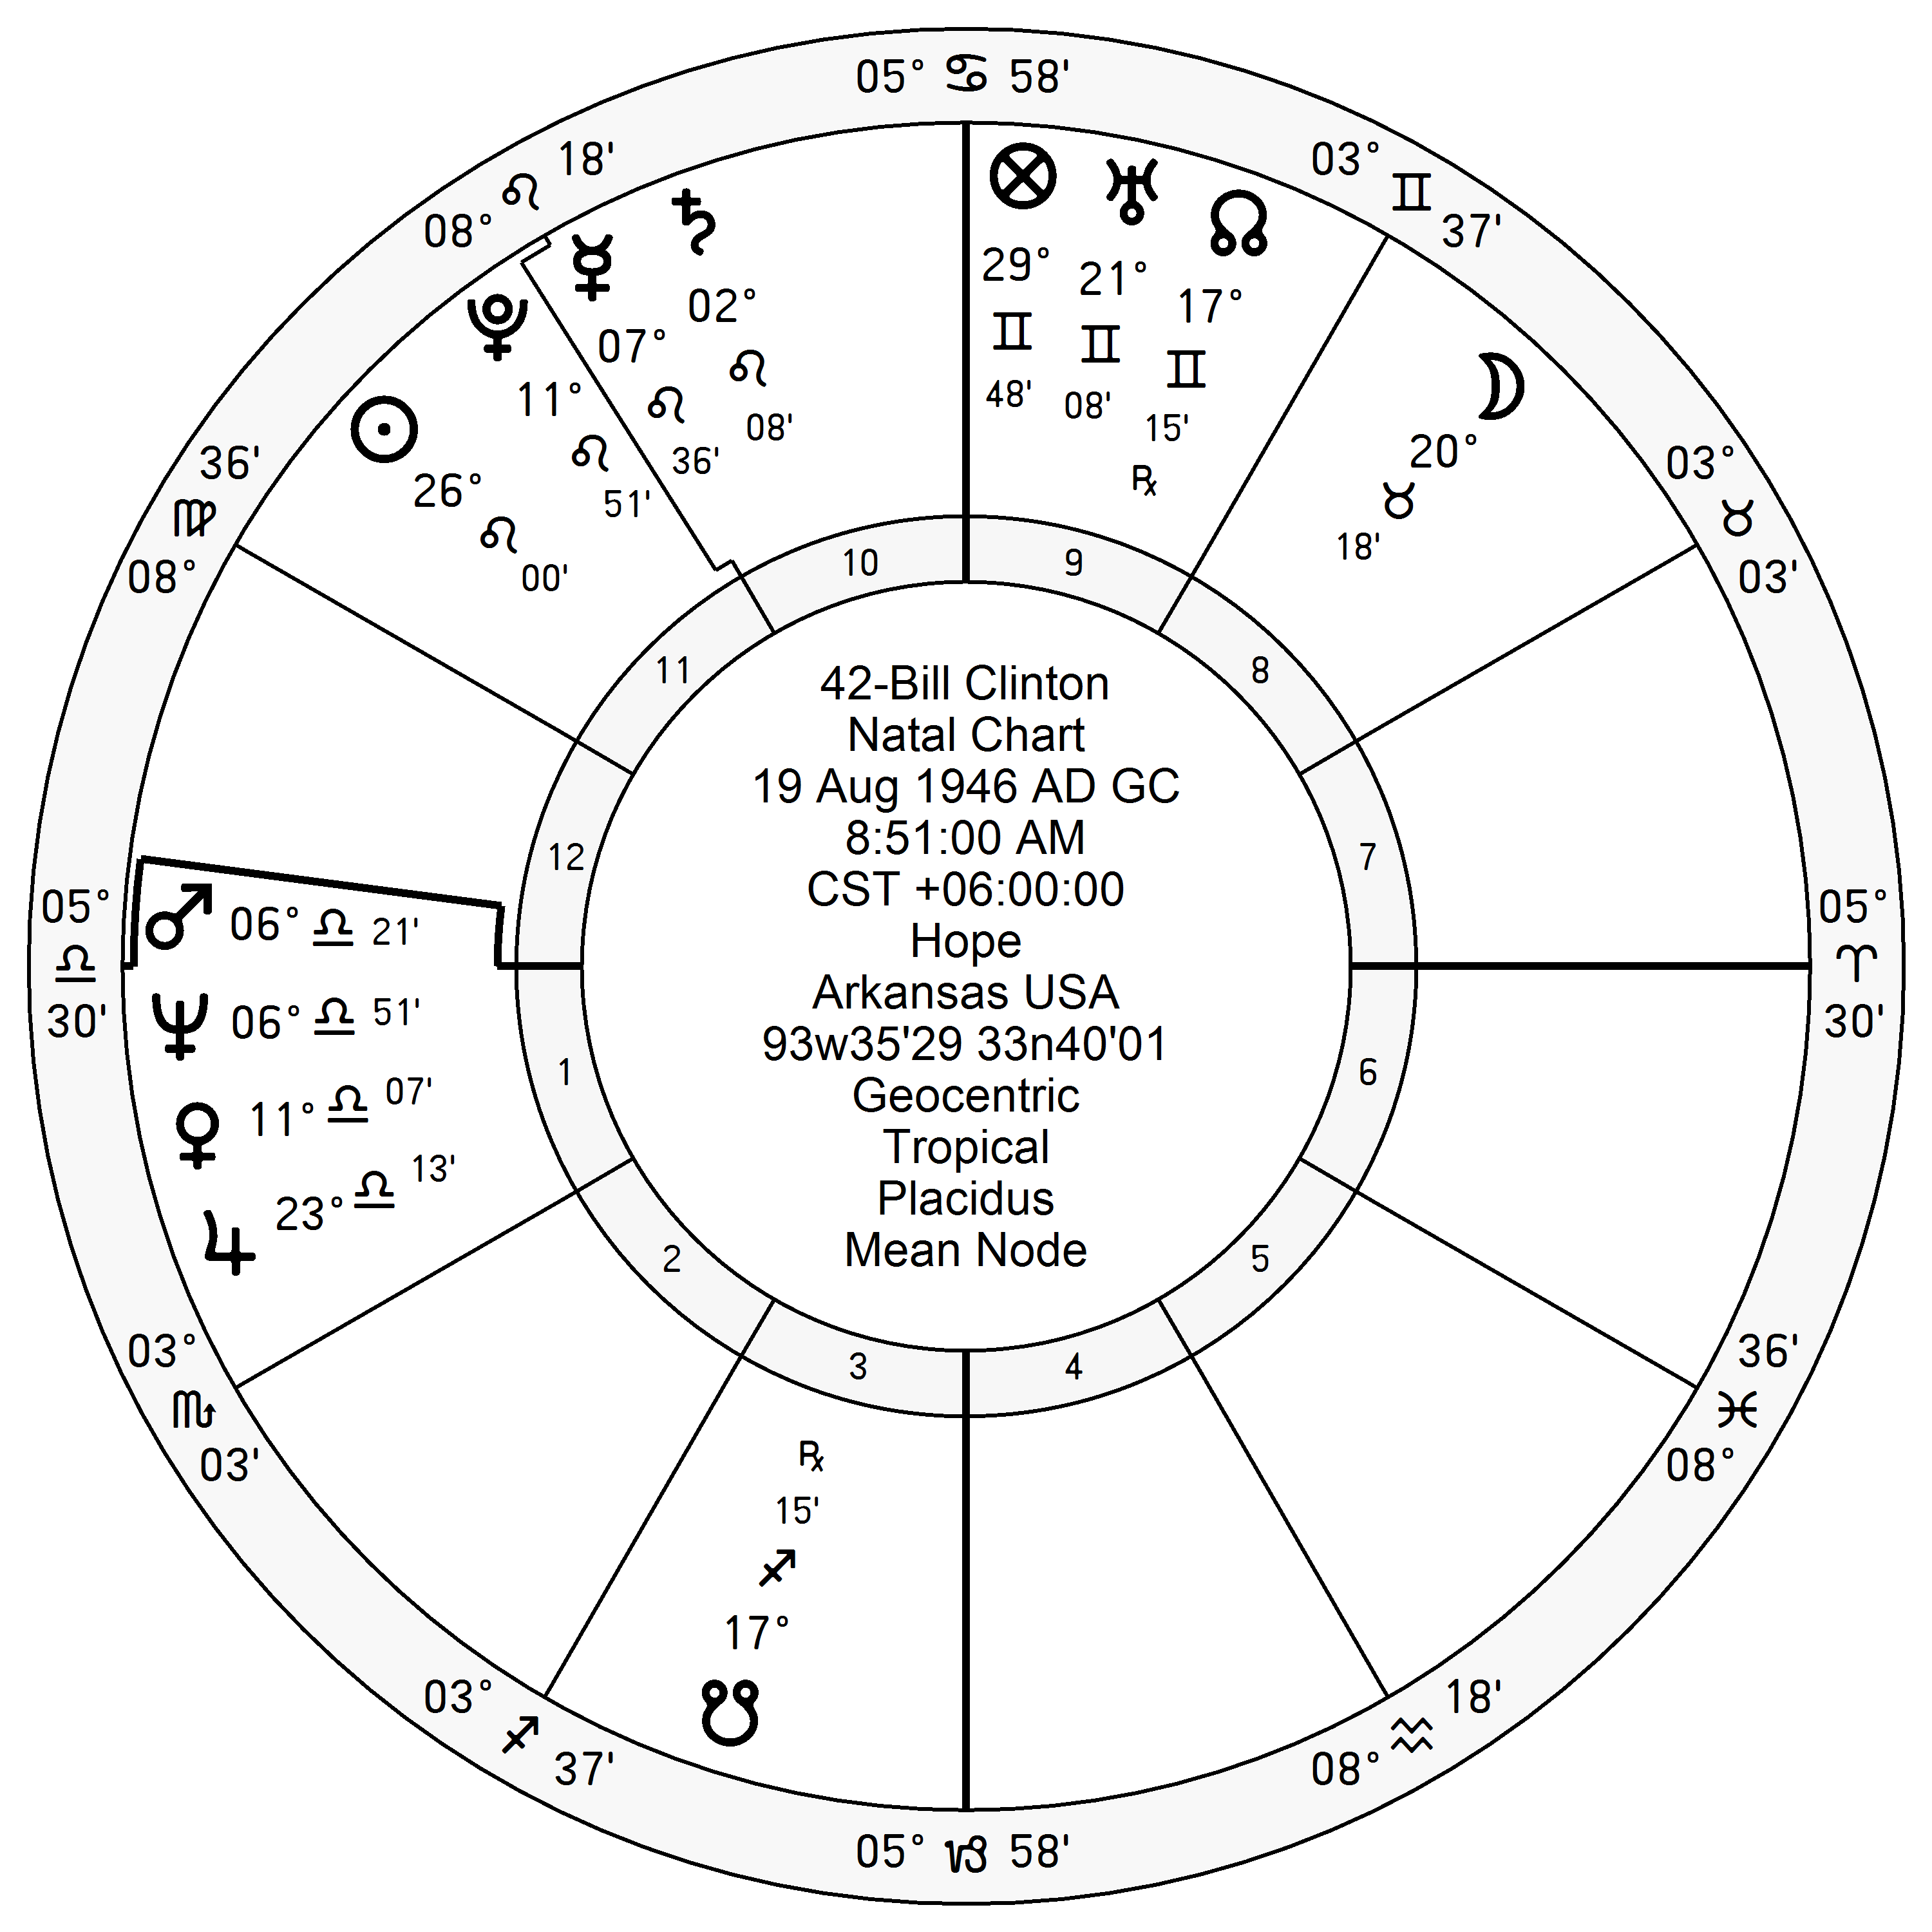
\includegraphics[width=0.9\textwidth]{charts/Clinton.png}}
\fontsize{8pt}{9pt}\selectfont

\Jupiter\, \Sextile\, P1; in N1 \Square\, N10 \\
\Mercury\, \Trine\, P1; in N10 \Sextile\, N1 \\
\Saturn\, in N10 \Sextile\, N1

\column{0.48\textwidth}
\vspace{-1em}
{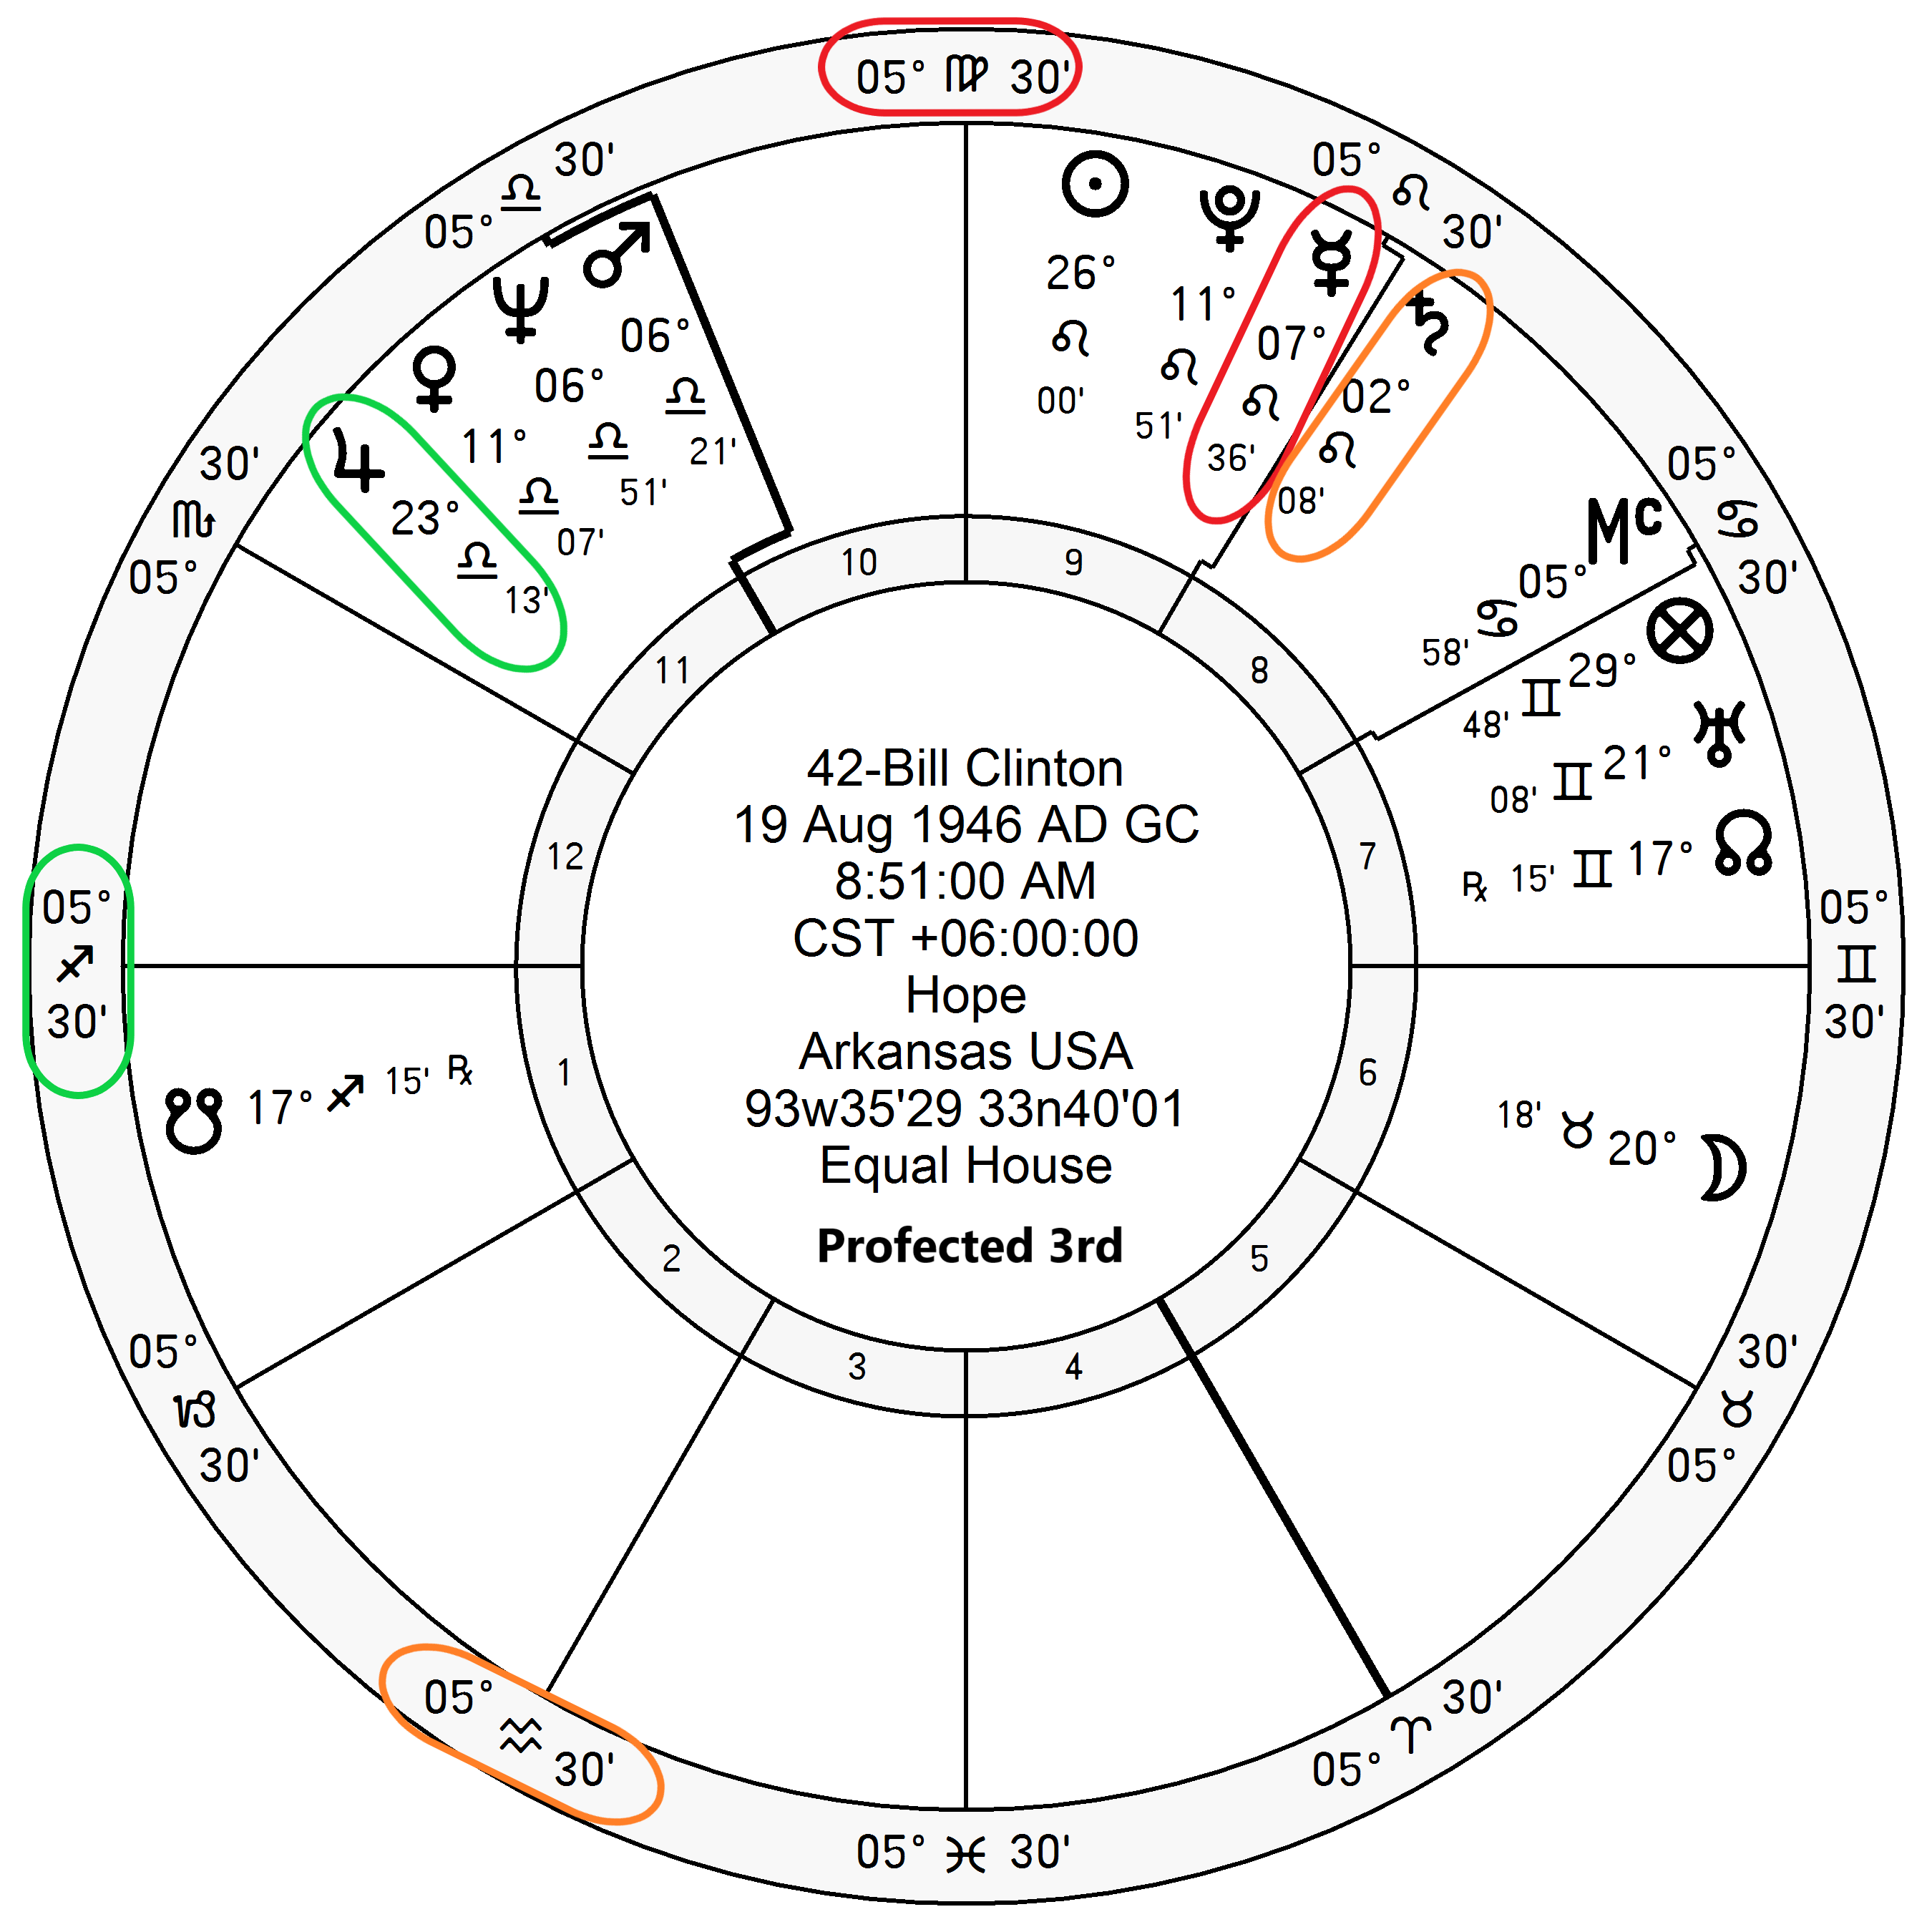
\includegraphics[width=0.9\textwidth]{charts/Clinton-Prof-3rd.png}}
\fontsize{8pt}{9pt}\selectfont

\textbf{\dgreen P1=N3}
	$\Rightarrow$ \Jupiter\, $\Rightarrow$ P11/\textbf{\dgreen N1}\\
\textbf{\red P10}=N12
	$\Rightarrow$ \Mercury\, $\Rightarrow$ P9/\textbf{\red N10}\\
PE=\textbf{\dgreen P3}/N5
	 $\Rightarrow$ \Saturn\, $\Rightarrow$ P8/\textbf{\red N10}

\end{columns}
\end{frame}

% ===================================================
\begin{frame}[t]{Election November 5, 1996: Robert Dole}
\small
\begin{columns}[T, onlytextwidth]
\column{0.48\textwidth}
\vspace{-1em}
{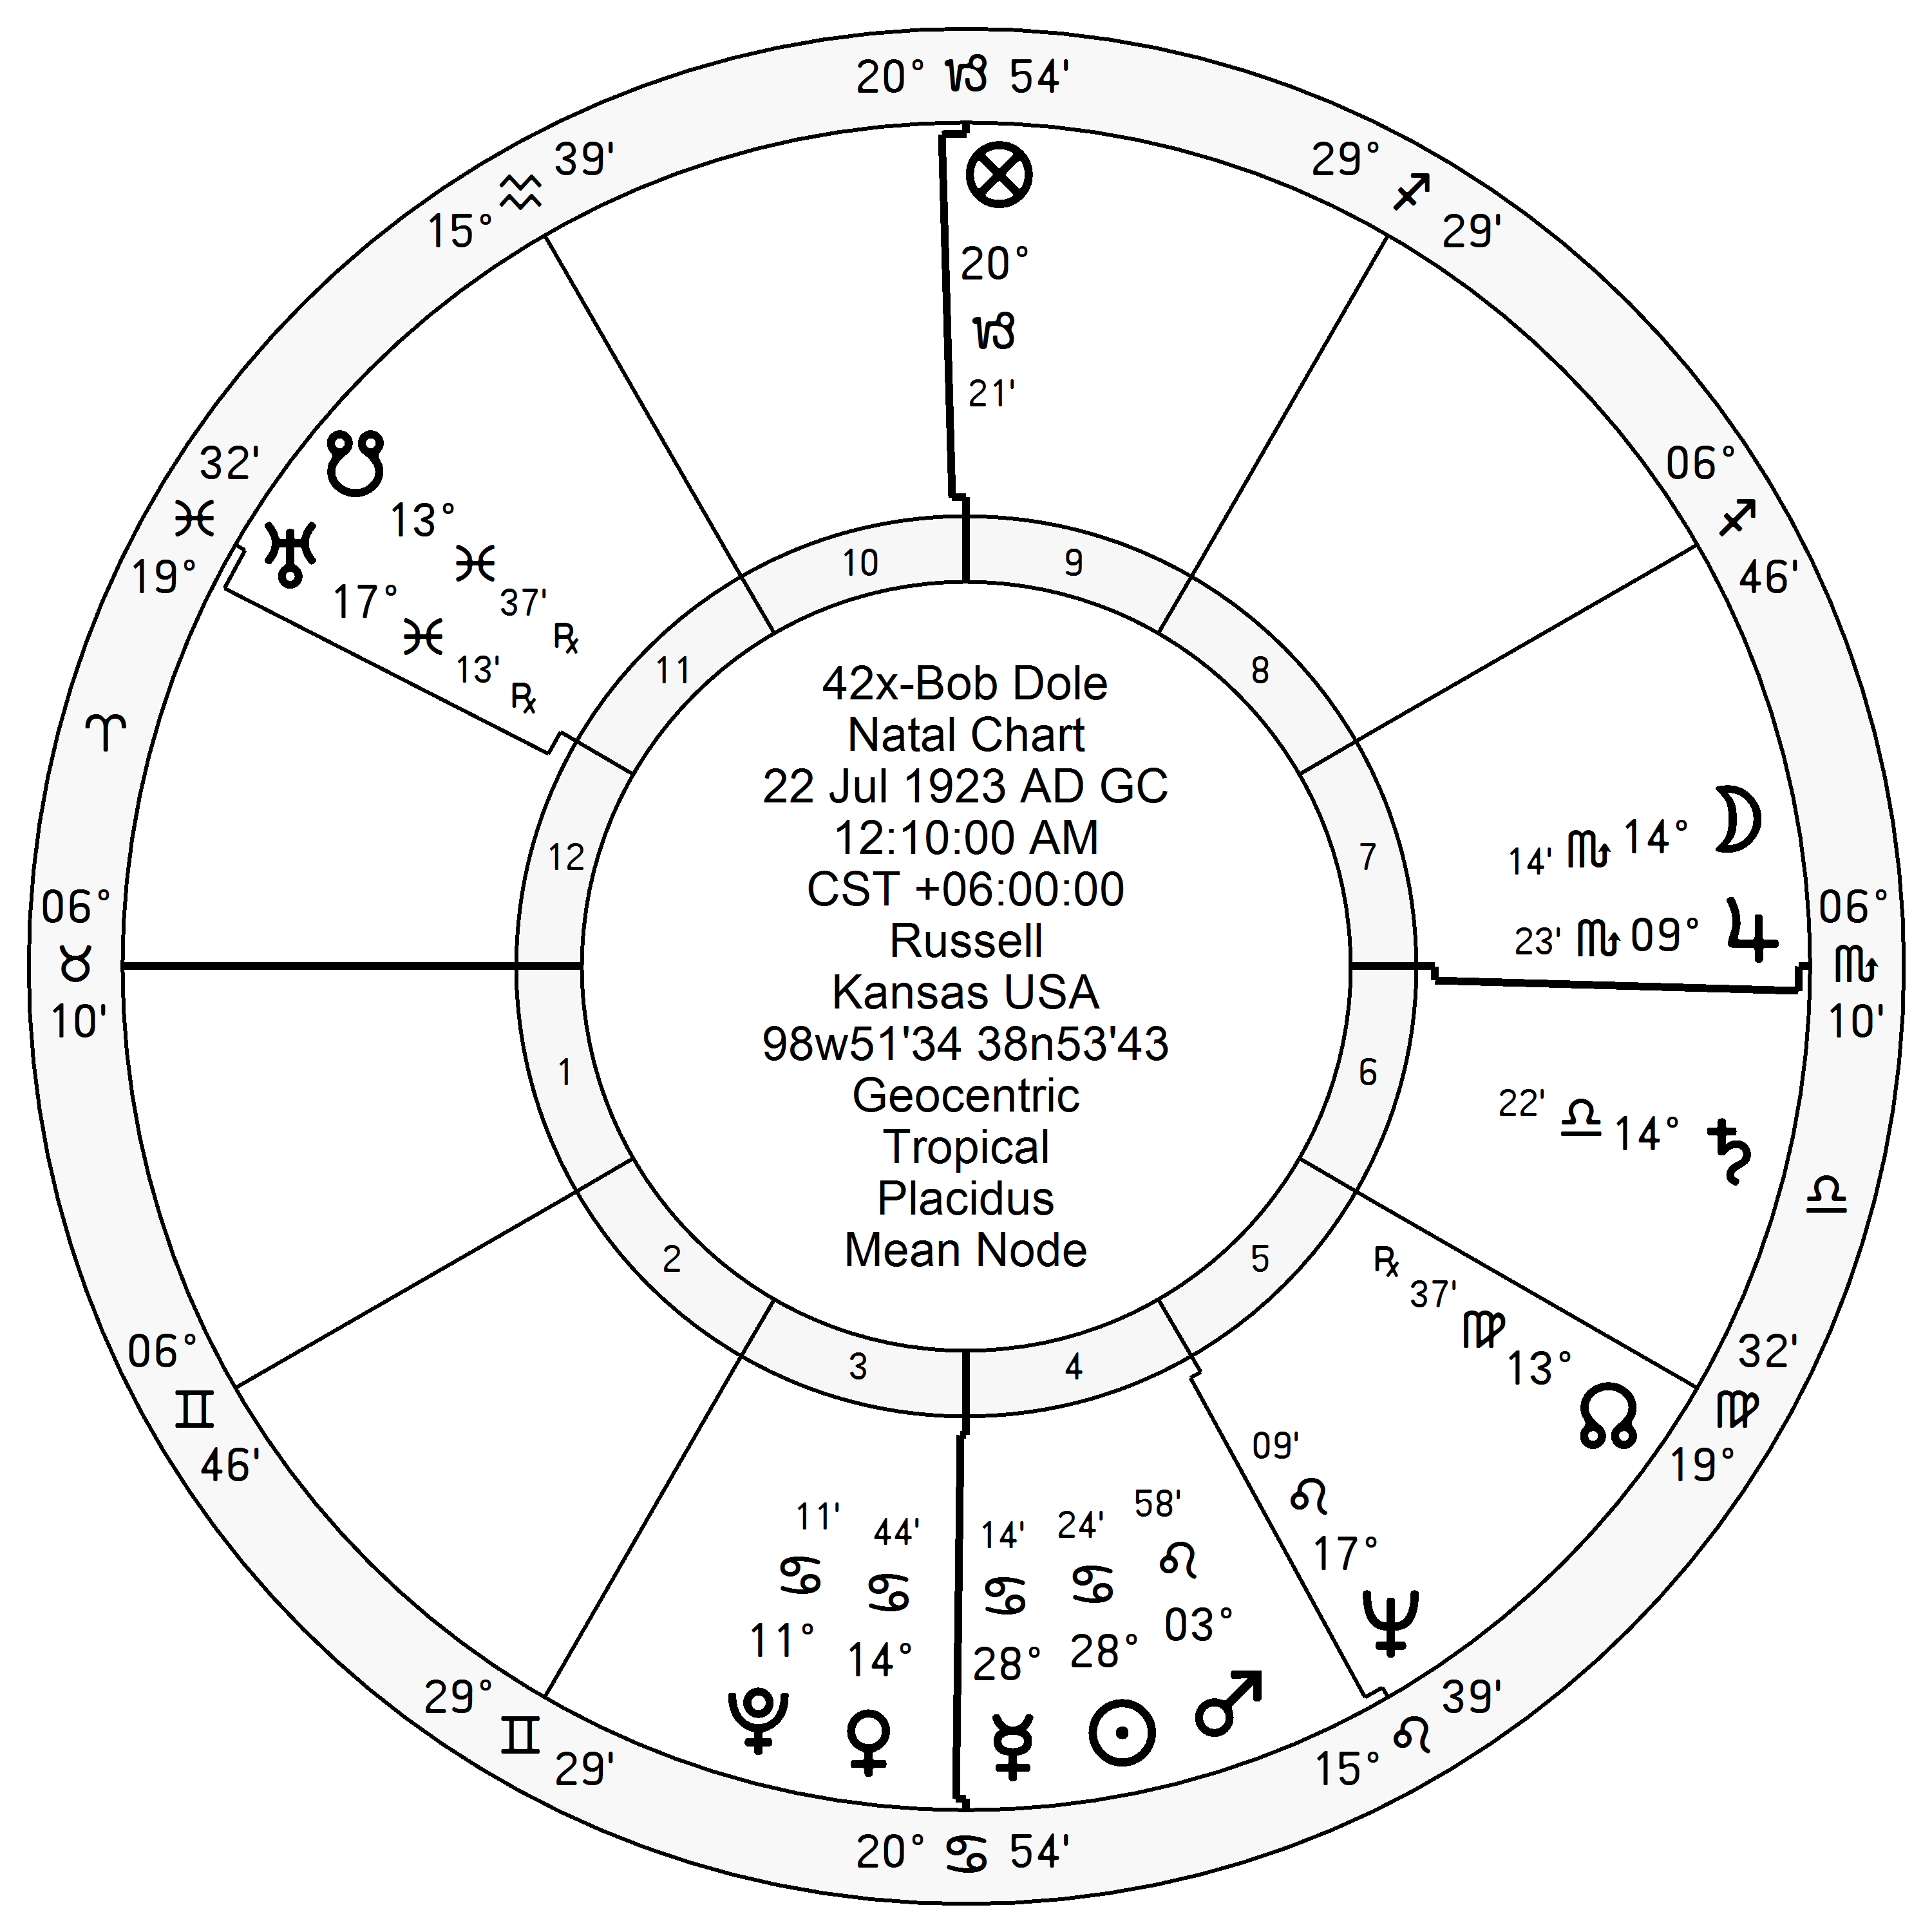
\includegraphics[width=0.9\textwidth]{charts/Dole.png}}

\Mercury\, (burnt) \Trine\, P10; \Opposition\, N10 \\
\Jupiter\, \Trine\, P10; \Opposition\, N1 \\
\vspace{0.5em}
Dole has a burnt \Mercury\, and the \SouthNode\, in the 10th working against him.


\column{0.48\textwidth}
\vspace{-1em}
{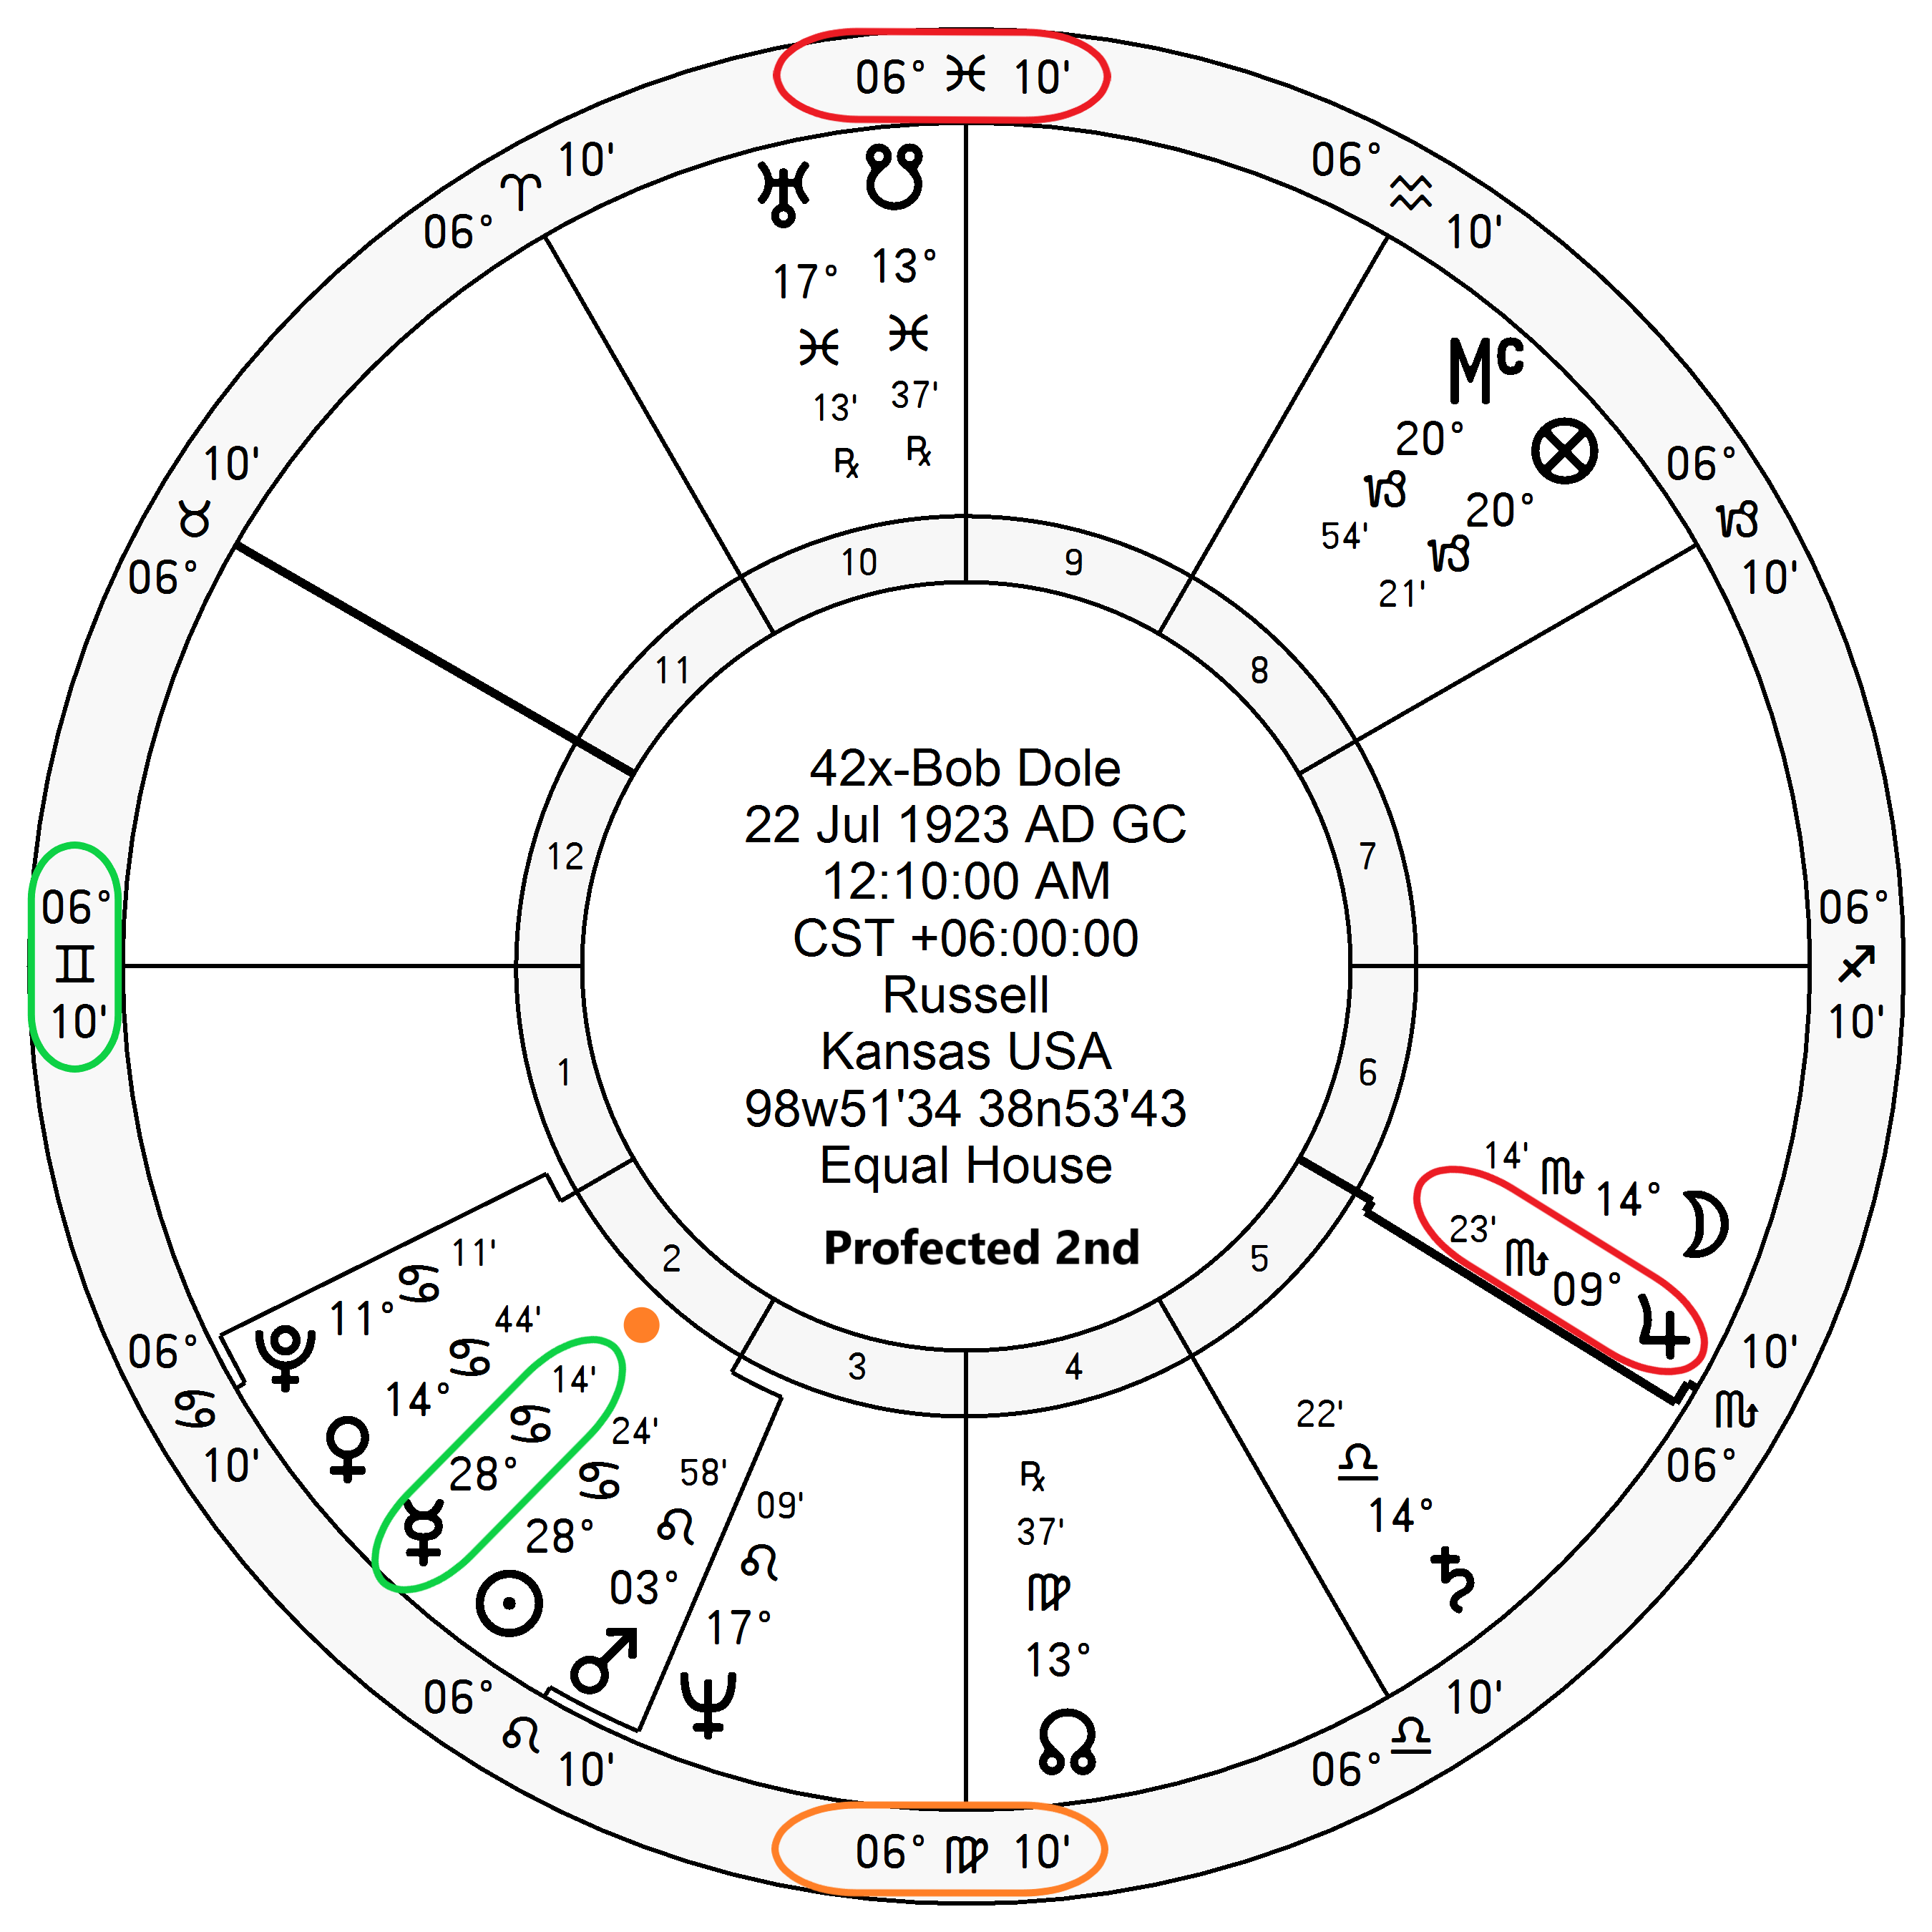
\includegraphics[width=0.9\textwidth]{charts/Dole-Prof-2nd.png}}
\fontsize{8pt}{9pt}\selectfont
\textbf{\dgreen P1}=N3
	$\Rightarrow$ \Mercury\, (burnt) $\Rightarrow$ \textbf{\dgreen P2/N4}\\
\textbf{\red P10}=N12
	$\Rightarrow$ \Jupiter\, $\Rightarrow$ \textbf{\red P6}/N7\\
PE=P4/\textbf{\red N6}
	 $\Rightarrow$ \Mercury\, (burnt) $\Rightarrow$ \textbf{\dgreen P2/N4}

\end{columns}
\end{frame}
